\documentclass[twocolumn,10pt,a4paper]{article}

\usepackage[url=false, doi=false,sorting=none]{biblatex}

\usepackage{lipsum}
\usepackage[scale=0.85]{geometry}
\usepackage{enumitem}
\usepackage{titlesec}
\usepackage{graphicx}
\usepackage{booktabs}
\usepackage[dvipsnames]{xcolor}
\usepackage{multirow}
\usepackage{array}
\usepackage{siunitx}
\usepackage{subcaption}
\usepackage[font=footnotesize,labelfont=bf]{caption}

\addbibresource{../bibliography.bib}

\titlelabel{}

\newcommand{\atom}[1]{\colorbox{Gray!30}{\ttfamily #1}}
\newcommand{\citen}[1]{~\parencite{#1}}
\newcommand{\citeay}[1]{\textcite{#1}}
\newcommand{\winner}[1]{{\bfseries\color{ForestGreen}#1}}

\newcommand{\mypycop}{\texttt{MyPyCoP}}
\newcommand{\pop}{\phantom{a}}
\newcommand{\cop}[1]{\textsf{#1}}

\pagenumbering{gobble}

\setlist[enumerate]{itemsep=1pt, topsep=1pt, parsep=0pt, partopsep=0pt}

\setcounter{footnote}{1}

\title{Vampire Post-Mortem}
\date{}
\author{}

\setlist{
	% itemsep=2pt,
	% topsep=0pt,
	% parsep=0pt,
	% partoparsep=0pt,
	leftmargin=10pt,
}

\begin{document}
\twocolumn[
	\centering
	\vspace{1em}
	{\LARGE\bfseries Vampire Paper Post-Mortem \par} \vspace{3pt}
	{\large (and next steps on my PhD) \par}
	\vspace{2em}
]

\section{Introduction}

The final paper was submitted to the Vampire workshop!
This is the first big win of my PhD, and the process of getting there allowed me to improve the core objectives that will be useful for writing the first-year report.

This one-pager presents some thoughts on the entire process to use as a guide for the report.

% \vspace{-25pt}

\section{Timeline}

% \vspace{-10pt}

\begin{description}
	\item[Michaelmas] \pop{}
		\begin{itemize}[label=---]
			\item Went over bibliography related to connection provers.
			\item Forked Fredrik's repo, and started experimenting with it.
			\item Created the \cop{ClassicalSAT} calculus on this fork, based on SATCoP\cite{eliminatingModels}.
		\end{itemize}
	\item[Lent] \pop{}
		\begin{itemize}[label=---]
			\item New, major fork in the connections prover (\mypycop{}).
			\item FOF translation in \mypycop{}.
			\item Figured out how to properly work the HPC. Created runner scripts to easily batch many experiments simultaneously.
			\item Strategies in \mypycop{}, and the \texttt{compare\_} \texttt{\_strategies.py} script.
			\item These two changes made it possible to test and iterate faster.
		\end{itemize}
	\item[Easter Vacation + Easter] \pop{}
		\begin{itemize}[label=---]
			\item Began writing weekly A4 papers during weekly meetings. Good idea!
			\item General experimentation in different areas.
				\begin{enumerate}
					\item Different schedulers, including using ParamILS\cite{hutterParamILSAutomaticAlgorithm2009}.
					\item \cop{PySATCoP} and \cop{PySATCoPLiteral}, strategy-level implementations of \cop{SATCoP}.
					\item Different cut-based policies: LeanCoP-style cuts, reduction-only cuts, \dots{}.
					\item Different reset policies.
					\item One-armed-bandit and reset-based policies.
					\item SAT-based features for tableau guidance.
				\end{enumerate}
			\item \textbf{April 29}: first version of the strategy that later became \cop{SATResetCoP}. Publishing this to FLoC became my main priority.
			\item Ran experiments on current environment to ensure the new strategy works correctly and there was no ``simpler'' competitor.
			\item \textbf{May 8 -- 28} Wrote Vampire paper.
			\item Worked with Fredrik to improve the paper and make it closer to the standard. Note that this is the first proper publication of the connections prover\cite{connections_2023}!
		\end{itemize}
\end{description}

\section{Thoughts and Questions}

\begin{itemize}
	\item Should I have spent less time experimenting and setting up the environment, and more time researching? I feel that ``wide'' paper discovery became a lot slower after Michaelmas, but I'm not sure how much I could have gained after reading the core papers.
	\item Did I get too focused on plots and tables? Maybe I should have done this at the end.
\begin{figure}[h]
	\fbox{
	\begin{minipage}{.45\columnwidth}
		\resizebox{\linewidth}{!}{
		  \begin{tabular}{@{}>{\ttfamily\bfseries}l l r S[table-format=5.0] S[table-format=6.0]@{}}
			  \toprule
			  {\rmfamily\bfseries Problem} & {\bfseries Strategy} & {\bfseries Solved} & {\bfseries Steps} & {\bfseries Time (ms)} \\
			  \midrule
			  \multirow{7}{*}{KRS255+1.p}
				  & \atom{SATSolve}                     & \texttt{false}  & 12659 & 90003 \\
				  & \atom{SATSolveGuided}               & \texttt{false}  &  9104 & 90002 \\
				  & \atom{SATSolveGuidedProbeConflicts} & \texttt{false}  & 10533 & 90002 \\
				  & \atom{SATSolveGuidedForcedTrue}     & \texttt{true} &  7423 & 40270 \\
				  & \atom{SATSolveGuidedEVSIDS}         & \texttt{true} &  6516 & 39185 \\
				  & \atom{SATSolveGuidedShort}          & \texttt{false}  & 13201 & 90007 \\
				  & \atom{SATSolveGuidedFast}           & \texttt{false}  & 12547 & 90011 \\
			  \addlinespace

			  \multirow{7}{*}{GEO214+2.p}
				  & \atom{SATSolve}                     & \texttt{false}  & 24308 & 90001 \\
				  & \atom{SATSolveGuided}               & \texttt{true} &  4831 &  4622 \\
				  & \atom{SATSolveGuidedProbeConflicts} & \texttt{false}  & 90966 & 90000 \\
				  & \atom{SATSolveGuidedForcedTrue}     & \texttt{false}  & 93502 & 90000 \\
				  & \atom{SATSolveGuidedEVSIDS}         & \texttt{false}  & 24030 & 90013 \\
				  & \atom{SATSolveGuidedShort}          & \texttt{true} & 15944 & 34071 \\
				  & \atom{SATSolveGuidedFast}           & \texttt{true} &  4440 &  3816 \\
			  \addlinespace

			  \multirow{7}{*}{SYN578-1.p}
				  & \atom{SATSolve}                     & \texttt{false}  & {--}  & {--} \\
				  & \atom{SATSolveGuided}               & \texttt{true} & 21388 & 103259 \\
				  & \atom{SATSolveGuidedProbeConflicts} & \texttt{true} & 11347 &  33783 \\
				  & \atom{SATSolveGuidedForcedTrue}     & \texttt{true} & 11994 &  32949 \\
				  & \atom{SATSolveGuidedEVSIDS}         & \texttt{false}  & {--}  & {--} \\
				  & \atom{SATSolveGuidedShort}          & \texttt{true} & 25291 & 100802 \\
				  & \atom{SATSolveGuidedFast}           & \texttt{true} & 11083 &  22460 \\
			  \addlinespace

			  \multirow{7}{*}{SYN583-1.p}
				  & \atom{SATSolve}                     & \texttt{false}  & {--}  & {--} \\
				  & \atom{SATSolveGuided}               & \texttt{true} & 13439 & 50791 \\
				  & \atom{SATSolveGuidedProbeConflicts} & \texttt{false}  & {--}  & {--} \\
				  & \atom{SATSolveGuidedForcedTrue}     & \texttt{false}  & {--}  & {--} \\
				  & \atom{SATSolveGuidedEVSIDS}         & \texttt{true} & 12521 & 46118 \\
				  & \atom{SATSolveGuidedShort}          & \texttt{true} & 13723 & 52979 \\
				  & \atom{SATSolveGuidedFast}           & \texttt{true} & 11991 & 37213 \\
			%   \addlinespace

			%   \multirow{7}{*}{SYN657-1.p}
			% 	  & \atom{SATSolve}                     & \texttt{false}  & {--}  & {--} \\
			% 	  & \atom{SATSolveGuided}               & \texttt{true} & 10996 & 60140 \\
			% 	  & \atom{SATSolveGuidedProbeConflicts} & \texttt{false}  & {--}  & {--} \\
			% 	  & \atom{SATSolveGuidedForcedTrue}     & \texttt{false}  & {--}  & {--} \\
			% 	  & \atom{SATSolveGuidedEVSIDS}         & \texttt{false}  & {--}  & {--} \\
			% 	  & \atom{SATSolveGuidedShort}          & \texttt{false}  & {--}  & {--} \\
			% 	  & \atom{SATSolveGuidedFast}           & \texttt{false}  & {--}  & {--} \\
			  \bottomrule
		  \end{tabular}
	  }
	\end{minipage}
	\begin{minipage}{.45\columnwidth}
		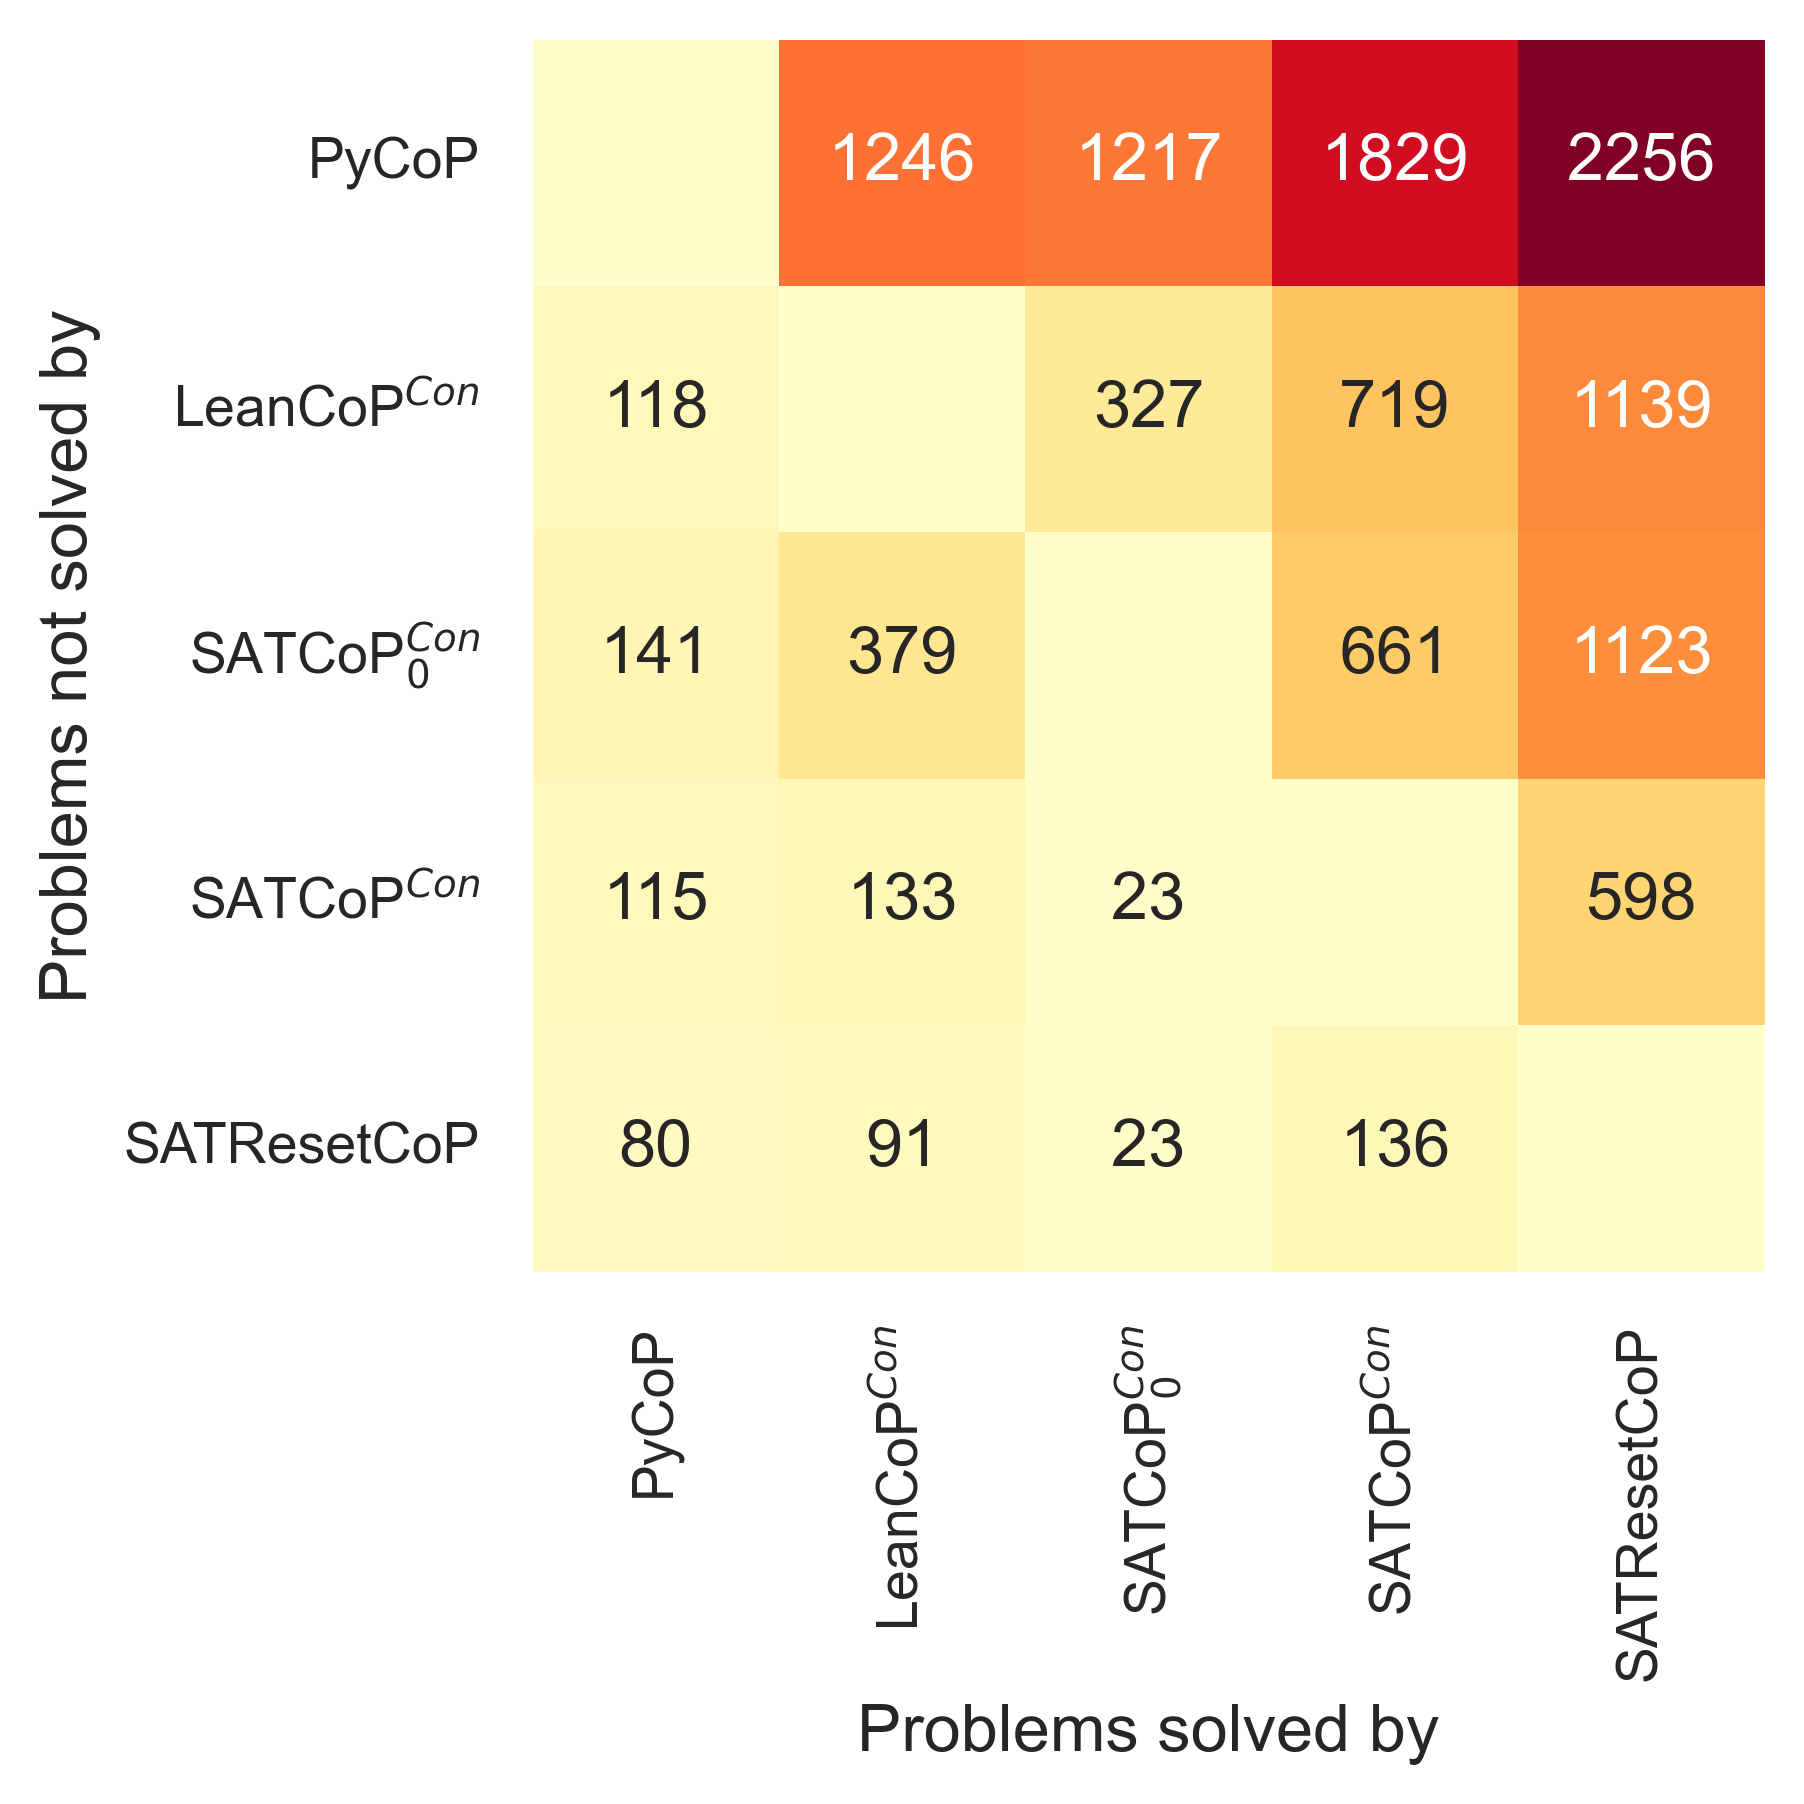
\includegraphics[width=\textwidth]{Vampire/figures/solved_heatmap.png}
	\end{minipage}
	}
	\caption{Example of the tables and plots I spent time producing. Were these the right level of analysis, or should I have left this for writing the paper?}
\end{figure} \vspace{-10pt}
	\item I should definitely have started working with Fredrik earlier.
		Big review last week before submission; he could also have helped me during experimentation.
	\item Focusing on building strong testing infrastructure \emph{first} was a great idea. Experimenting quickly is always good.
	\item I'm not sure how I could have made it on time for the UNIF workshop. Would it make sense to keep a few experiments ``in reserve'' waiting for these deadlines?
\end{itemize}

\section{Next Steps}

\begin{enumerate}
	\item Current priority: \textbf{First-year Report}. Deadline June~30th, so not a lot of time to go.
	\item Let's send the current tableau prover to CASC! I'll start the work on this soon.
	\item How different does this paper have to be to send these experiments to another conference or journal?
\end{enumerate}

\renewcommand*{\bibfont}{\tiny}
\printbibliography[title={Tiny References}]{}

\end{document}
